% =============================================================================
% CMP719 Computer Vision — Final Report (v2)
% Scene-SKDE: a multi-agent keypoint-density extension of SeeKer for
% pedestrian-vehicle hazard detection.
% ICLR 2025 template. Compile: pdflatex main && pdflatex main
% =============================================================================
\documentclass{article}
\usepackage{iclr2025_conference,times}

\usepackage{amsmath,amssymb,amsthm}
\usepackage{graphicx}
\usepackage{booktabs}
\usepackage{hyperref}
\usepackage{url}
\usepackage{xcolor}

\graphicspath{{figures/}}

\title{Scene-SKDE: A Multi-Agent Keypoint-Density Extension of SeeKer\\
       for Pedestrian--Vehicle Hazard Detection \\ \vspace{0.4em}
       {\large CMP719 Computer Vision --- Final Report}}

\author{Doruk Topcu \\
        Department of Computer Engineering \\
        Hacettepe University \\
        \texttt{N25142281}}

\iclrfinalcopy
\begin{document}
\maketitle

\begin{abstract}
The Sequential Keypoint Density Estimator (SeeKer/SKDE, ICCV~2025) is a
deliberately simple yet strong baseline for skeleton-based video anomaly
detection: it models a pedestrian's 2D keypoint trajectory with an
autoregressive density and flags low-likelihood motion. It is, however,
\emph{environmentally blind} --- each skeleton is scored in isolation, so a
pedestrian walking calmly and the same pedestrian walking into a vehicle's path
receive identical scores. We extend SeeKer to the \emph{multi-agent} scene.
Each vehicle is encoded as a compact oriented-keypoint set (an oriented bounding
box rendered as four corners, a centre and a heading), and is either injected as
a per-frame context (with an optional FiLM covariance gate) or, in our headline
\emph{Scene-SKDE}, concatenated with the pedestrian into a single skeleton of
$N'{=}18{+}6M$ keypoints modelled under one autoregressive factorisation. On the
ShanghaiTech Campus dataset, the context model improves the baseline by
$+6.0$ percentage points of mean frame-AUROC over five seeds
($0.726\!\rightarrow\!0.786$, highly significant). More importantly, a
\emph{counterfactual} probe --- re-scoring with the vehicle ``removed'' ---
shows the gain is a configuration-dependent pedestrian--vehicle \emph{interaction}
signal that the pedestrian-only baseline structurally cannot produce
(near-vehicle-hazard AUROC $0.79\!\rightarrow\!0.97$; score--proximity
correlation $0.16\!\rightarrow\!0.70$), rather than mere object presence. We also
report honestly: the overall-AUROC advantage narrows under temporal score
smoothing, and a full presence-vs-interaction separation requires a benchmark
where vehicles are sometimes normal. Our contribution is the multi-agent
generalisation of an autoregressive keypoint density and the demonstration of an
isolated interaction signal, supported by a reproducible, error-barred
evaluation.
\end{abstract}

% =============================================================================
\section{Introduction and Problem Statement}
\label{sec:intro}

Video anomaly detection (VAD) identifies events that deviate from normal
training behaviour. Skeleton-based VAD operates on 2D human poses rather than
RGB pixels, gaining low dimensionality, appearance/lighting invariance, and
privacy~\citep{morais2019messagepassing,markovitz2020graph,hirschorn2023normalizing}.
Within this family, SeeKer~\citep{delic2025seeker} factorises a pedestrian's
pose sequence with a masked autoregressive network (MADE,
\citealp{germain2015made}) and scores anomalies by negative log-likelihood
(NLL); despite its simplicity it rivals heavier graph- and flow-based models.

\paragraph{The problem.} SeeKer conditions only on a pedestrian's \emph{own}
past keypoints and aggregates multiple people by a per-frame maximum --- it
never observes other agents. Yet in traffic-hazard surveillance the anomaly is
rarely the gait in isolation; it is the \emph{interaction} --- a pedestrian too
close to, or in the path of, a vehicle. A motion-only density cannot represent
this: the two situations above are equally likely under it. We ask whether
SeeKer's elegant keypoint-density formulation can be extended to model the
\emph{scene} --- pedestrians \emph{and} vehicles --- so that one likelihood-based
score reflects pedestrian--vehicle interaction.

\paragraph{Contributions.} We frame our claims around what the evidence supports.
\begin{itemize}\itemsep2pt
  \item \textbf{Scene-SKDE: a multi-agent keypoint density.} We generalise
  SeeKer from a single human skeleton to a joint scene of road agents. Each
  vehicle becomes a compact oriented-keypoint set and is modelled \emph{together}
  with the pedestrian under one autoregressive factorisation, with the pedestrian
  predicted \emph{given} the surrounding vehicles. To our knowledge this is the
  first multi-agent extension of this estimator (Section~\ref{sec:method}).
  \item \textbf{Context-conditioned variant with FiLM covariance.} A lighter
  alternative injects the vehicle geometry as a per-frame context through an
  autoregressive-preserving shortcut and a FiLM head~\citep{perez2018film} that
  lets the context modulate the predicted covariance.
  \item \textbf{Evidence of interaction, not object presence.} A counterfactual
  probe isolates the vehicle's effect on the pedestrian likelihood and shows it is
  a configuration-dependent interaction signal (Section~\ref{sec:results}).
  \item \textbf{Honest, reproducible evaluation.} Multi-seed mean$\pm$std, a
  hazard-subset analysis, a careful operating-point study, and a frank
  limitations section.
\end{itemize}

% =============================================================================
\section{Related Work}
\label{sec:related}

\paragraph{Skeleton-based VAD.} \citet{morais2019messagepassing} introduced
recurrent message passing over joints; \citet{markovitz2020graph} clustered
spatio-temporal graph embeddings; STG-NF~\citep{hirschorn2023normalizing} fits a
normalizing flow over joint graphs. SeeKer~\citep{delic2025seeker} shows a
masked autoregressive density (MADE,~\citealp{germain2015made}) is a strong,
overlooked baseline; we build directly on it. Exact-likelihood flows
(RealNVP~\citealp{dinh2017realnvp}, Glow~\citealp{kingma2018glow}) are the
natural route to a more expressive conditional (Section~\ref{sec:future}).

\paragraph{Context- and interaction-aware VAD.} A separate strand injects
scene/object cues: \citet{ionescu2019object} score per-object features with
one-class SVMs. Closest to us are interaction methods:
\citet{wiederer2022anomaly} model a density over multiple road-agent trajectories
and flag low-density configurations, and ComplexVAD~\citep{complexvad2025}
targets ``complex'' anomalies arising from the interaction of two or more
actors. These operate on trajectory/graph features. Our mechanism is orthogonal:
we keep SeeKer's autoregressive \emph{keypoint} density and widen its support to
multiple, heterogeneous agents within one factorisation. The vehicle
representation is an oriented bounding box rendered as keypoints --- not an
articulated skeleton; we use ``skeleton'' only by analogy.

% =============================================================================
\section{Method}
\label{sec:method}

\subsection{Baseline: SeeKer in brief}
A track is a sequence of frames, each with $V{=}18$ COCO-18 2D keypoints. Let
$X_{t,n}\!\in\!\mathbb{R}^2$ be keypoint $n$ of frame $t$, $X_{t,<n}$ the earlier
keypoints of the same frame, and $X_\Delta$ all keypoints of the previous
$\Delta$ frames. SeeKer factorises
\begin{equation}
\label{eq:seeker}
p_\theta(X_t\mid X_\Delta)=\prod_{n=1}^{V} p_\theta\!\left(X_{t,n}\mid X_{t,<n},X_\Delta\right),
\quad
p_\theta(X_{t,n}\mid\cdot)=\mathcal{N}(\mu_\theta,\Sigma_\theta).
\end{equation}
Following SeeKer's headline configuration (and the released code), $\Sigma_\theta$
is \emph{diagonal}; a single masked network outputs $\mu_\theta$ and a per-axis
log-variance. (SeeKer ablates a full $2{\times}2$ Cholesky covariance but reports
it on par with diagonal, $77.8$ vs $77.9$ on UBnormal, so we keep the diagonal
form.) The anomaly score is the confidence-weighted NLL
$s(X_t)=-\sum_n c_{t,n}\ln p_\theta(X_{t,n}\mid X_{t,<n},X_\Delta)$, and the
per-frame score is the maximum over people --- i.e.\ people are modelled
\emph{independently}, with no object or interaction terms.

\subsection{Vehicles as oriented keypoints}
\label{ssec:carmatrix}
For each frame we run YOLOv11 segmentation on the raw image and keep the hazard
classes (\texttt{car, bus, truck, motorcycle, bicycle}). From each instance mask
we fit an oriented rectangle (\texttt{cv2.minAreaRect}) and read off $K_v{=}6$
keypoints: the four oriented corners, the centre, and a heading point along the
major axis. Crucially these are computed in \emph{pixel} space and then
normalised, so orientation is faithful (rotating an oriented box in
anisotropically-normalised coordinates would distort angles).

\paragraph{Coordinate-frame consistency.} A subtle but decisive detail: the
pedestrian reference used to make the representation translation/scale-invariant
must live in the \emph{same} frame as the detections. SeeKer normalises each pose
segment to zero mean and unit variance, which destroys absolute image position;
computing the pedestrian centroid from that normalised pose makes the context
\emph{pedestrian-independent}. We instead take the centroid from the raw pixel
keypoints divided by the frame size, placing it in the same $[0,1]$ image frame
as the YOLO boxes. Each vehicle keypoint is then expressed relative to the
pedestrian centroid and divided by the pedestrian's scale.

\subsection{Two ways to use the vehicles}
\paragraph{(a) Context-conditioned CCSKDE.} We append the per-frame vehicle
representation $C_t$ (either a per-class proximity vector, or the oriented
``car matrix'' of Section~\ref{ssec:carmatrix}) to MADE's input as an
\emph{unconditional shortcut}: its columns in the input mask are all-ones, so
every hidden unit may read every entry of $C_t$ while the keypoint-to-keypoint
causality is bit-for-bit preserved. A FiLM head~\citep{perez2018film} maps $C_t$
to per-coordinate $(\gamma,\beta)$ that gate the predicted log-variance,
$\log\sigma^2\leftarrow(1{+}\gamma(C_t))\log\sigma^2+\beta(C_t)$, realising a
\emph{contextual covariance penalty}; it is zero-initialised, so training begins
exactly at the shortcut-only model.

\paragraph{(b) Unified Scene-SKDE.} Our headline model treats vehicles as
first-class agents. We form one scene skeleton
\begin{equation}
\label{eq:scene}
Z_t=[\,V^1_t,\dots,V^M_t,\;P_t\,]\in\mathbb{R}^{N'\times 2},\qquad N'=18+6M,
\end{equation}
concatenating the $M$ nearest vehicle keypoint sets $V^m_t$ with the pedestrian
$P_t$, vehicles ordered \emph{first}, and normalised \emph{jointly}. SeeKer's
factorisation~(Eq.~\ref{eq:seeker}) is applied verbatim to $Z$, giving one scene
density and one hazard score
\begin{equation}
\label{eq:scene_score}
S(t)=-\sum_{n=1}^{N'} c_{t,n}\,\ln p_\theta\!\left(Z_{t,n}\mid Z_{t,<n},Z_\Delta\right).
\end{equation}
Because vehicles precede the pedestrian in the order, each pedestrian keypoint is
predicted \emph{given} the surrounding vehicles --- the interaction is captured by
the conditioning. (An ablation in Section~\ref{sec:ablation} shows that, for the
unified model, it is the joint inclusion of the vehicles more than this specific
ordering that drives the effect.) For frame-level comparability we read out the pedestrian
keypoint terms (the last 18), which already reflect the vehicle conditioning. The
masked network is the same MADE with its keypoint count generalised from $18$ to
$N'$. We verify by an autograd Jacobian sweep that no keypoint depends on an
equal- or later-ordered keypoint of the same frame (\textbf{0} forbidden-region
violations), while pedestrian keypoints \emph{can} attend to vehicle keypoints
--- the interaction pathway.

\paragraph{Scope of the density.} Conditioning is first-order
(pedestrian-given-vehicles) and, with a diagonal Gaussian, each conditional is
unimodal; genuinely multimodal normal behaviour (passing either side of a parked
car) is only approximated. We revisit this in Section~\ref{sec:limitations}.

\begin{figure}[t]
\centering
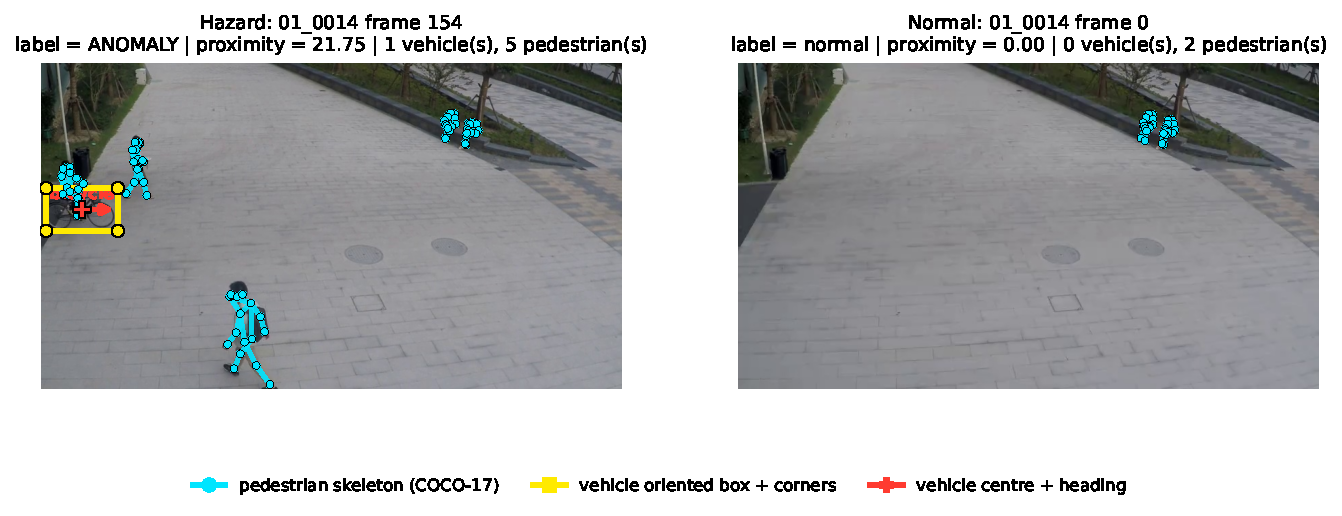
\includegraphics[width=0.98\textwidth]{qualitative.pdf}
\caption{\textbf{The scene representation on real ShanghaiTech test frames.}
\emph{Left:} an anomalous near-vehicle frame --- the pedestrian skeleton (cyan,
COCO-17) sits directly against the vehicle's oriented-keypoint set (yellow box
corners; red centre and heading arrow), the pedestrian--vehicle
\emph{configuration} our Scene-SKDE conditions on. \emph{Right:} a normal frame
from the same scene with no vehicle present. The motion-only baseline sees only
the cyan skeletons and scores both situations identically; Scene-SKDE additionally
conditions the pedestrian keypoints on the yellow/red vehicle keypoints.}
\label{fig:qual}
\end{figure}

% =============================================================================
\section{Datasets and Exploratory Analysis}
\label{sec:data}

We use ShanghaiTech Campus~\citep{liu2018future}: 13 outdoor scenes, 330 training
and 107 test videos. Anomalies (cycling/driving in pedestrian zones, etc.) are
typically pedestrian--object interactions, making it the natural benchmark for our
hypothesis. Poses are AlphaPose~\citep{fang2017rmpe} COCO-17 keypoints converted
to COCO-18 (we use the STG-NF release for reproducibility); vehicles are obtained
once, offline, with YOLOv11~\citep{ultralytics2024yolov11} segmentation. The test
split comprises $40{,}791$ frames, of which $17{,}326$ ($42.5\%$) are anomalous
and $5{,}576$ contain at least one detected hazard.

\begin{figure}[t]
\centering
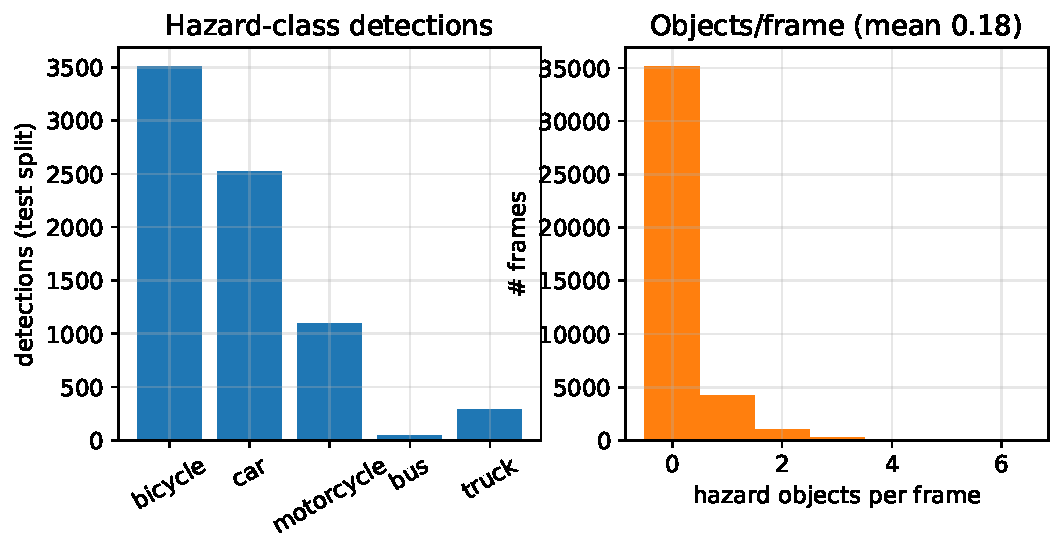
\includegraphics[width=0.49\textwidth]{eda_vehicle_classes.pdf}\hfill
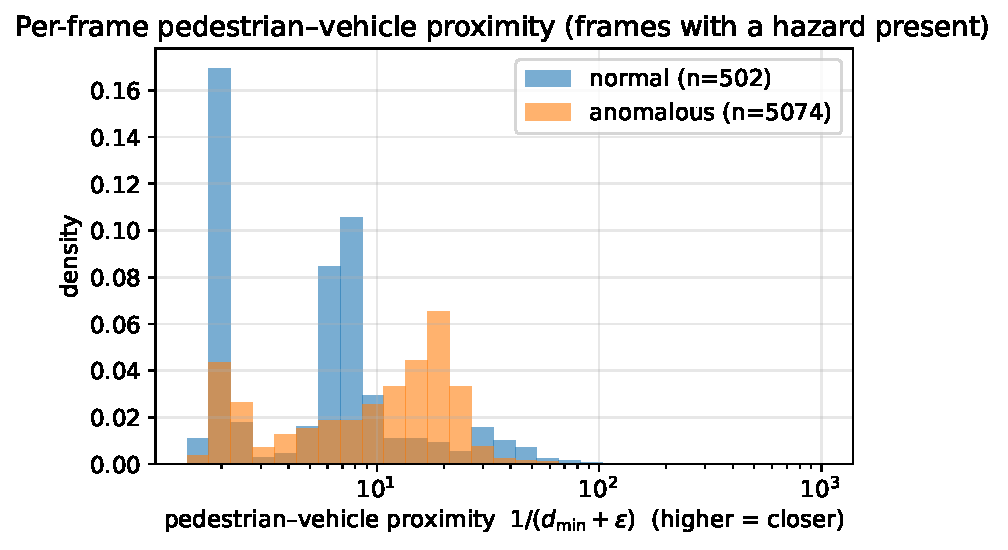
\includegraphics[width=0.49\textwidth]{eda_proximity_hist.pdf}
\caption{\textbf{Dataset EDA.} \emph{Left:} hazard-class detection counts and the
distribution of detected objects per frame (most frames contain none --- vehicles
are rare on a pedestrian campus). \emph{Right:} the distribution of per-frame
pedestrian--vehicle proximity $1/(d_{\min}{+}\epsilon)$ for frames where a hazard
is present, split by label; anomalous frames concentrate at \emph{higher}
proximity (closer pedestrian--vehicle configurations).}
\label{fig:eda1}
\end{figure}

\begin{figure}[t]
\centering
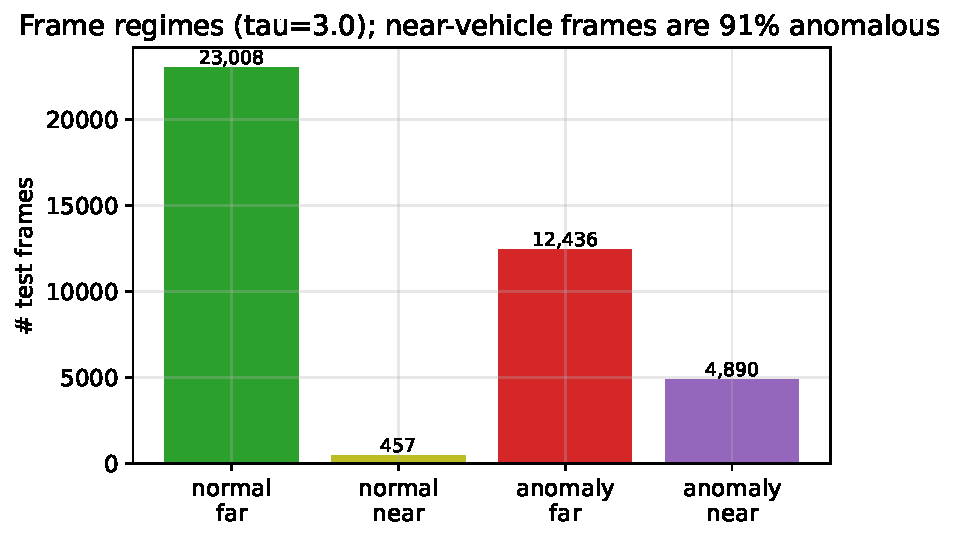
\includegraphics[width=0.62\textwidth]{eda_regime_breakdown.pdf}
\caption{\textbf{Frame-regime breakdown.} Among the few frames where a vehicle is
near a pedestrian, the overwhelming majority are \emph{anomalous}
($\sim$91\%). On ShanghaiTech a vehicle near a pedestrian almost \emph{is} the
anomaly --- which both motivates a hazard-focused evaluation and warns that this
benchmark cannot, by itself, separate ``hazard'' from ``object presence''
(Section~\ref{sec:limitations}).}
\label{fig:eda2}
\end{figure}

Figures~\ref{fig:eda1}--\ref{fig:eda2} summarise three observations that shape our
evaluation: (i) hazard objects are \emph{rare} (most frames have none), so a
detector that simply reacts to vehicle presence already correlates with the
label; (ii) when a hazard is present, anomalous frames sit at closer
pedestrian--vehicle distances; and (iii) near-vehicle frames are $\sim$91\%
anomalous, a near-degenerate subset that makes a naive ``within-interaction''
AUROC unstable and motivates the class-balanced and counterfactual metrics below.

% =============================================================================
\section{Experimental Setup}
\label{sec:setup}
All models train on normal sequences only, minimising the NLL of
Eq.~\ref{eq:seeker}/\ref{eq:scene_score}: 10 epochs, batch 1024, segment length
24, stride 1, Adam at $5{\times}10^{-4}$, a single-layer MADE (expansion 1), on a
single NVIDIA RTX~5080. Scoring is unchanged from SeeKer (confidence-weighted
per-keypoint NLL, max over people, temporal smoothing $\sigma$). We report
frame-level AUROC, AUPRC and EER, a \emph{per-scene} macro-AUROC, and ---
because overall AUROC mixes motion-intrinsic with interaction anomalies --- a
hazard-focused suite: a class-balanced near-vehicle AUROC (bootstrap CI), the
Spearman correlation between score and pedestrian--vehicle proximity, and a
counterfactual interaction probe (Section~\ref{sec:results}). For significance we
use both a seed-level $t$-test (five seeds $\{42,1,2,3,4\}$) and, on identical
test frames, DeLong's correlated-AUC test with a \emph{clip-level} block bootstrap
that respects within-clip temporal correlation.

% =============================================================================
\section{Results}
\label{sec:results}

\paragraph{Overview (single seed).} Table~\ref{tab:single} and
Figure~\ref{fig:epoch} compare all variants. Every context/scene variant lifts
the baseline by $+6$--$7$ pp of \emph{mean} AUROC. The corrected proximity
context and the richer oriented car-matrix perform comparably ($0.803$ vs
$0.802$ best); FiLM gives the best mean ($0.790$); and the unified Scene-SKDE
matches them ($0.798$ best) through a single, more principled formulation.

\begin{table}[t]
\centering
\caption{ShanghaiTech validation AUROC, single seed (10 epochs). All rows share
one reproduced baseline and one evaluation pipeline.}
\label{tab:single}
\begin{tabular}{lcc}
\toprule
Model & Best AUROC & Mean AUROC \\
\midrule
SeeKer baseline & 0.7351 & 0.7204 \\
CCSKDE proximity (coord-corrected) & \textbf{0.8034} & 0.7857 \\
CCSKDE car-matrix (oriented vehicle kpts) & 0.8023 & 0.7855 \\
CCSKDE car-matrix + FiLM & 0.7971 & \textbf{0.7898} \\
\;\;\emph{car-matrix, shuffled context (control)} & 0.7893 & 0.7835 \\
\midrule
\textbf{Unified Scene-SKDE} & 0.7980 & 0.7863 \\
\bottomrule
\end{tabular}
\end{table}

\begin{figure}[t]
\centering
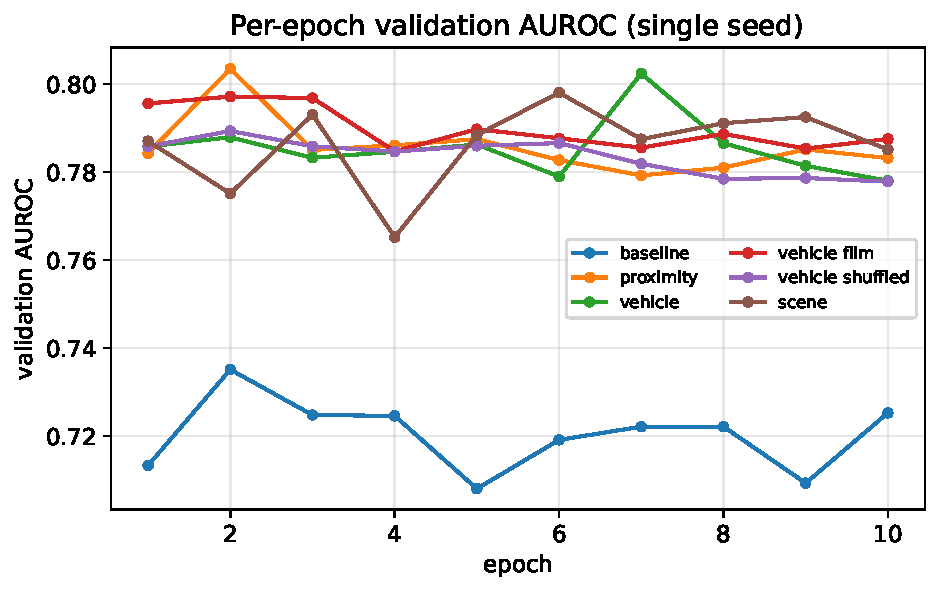
\includegraphics[width=0.62\textwidth]{res_epoch_curves.pdf}
\caption{\textbf{Per-epoch validation AUROC} (single seed). The baseline (lowest
band) is separated from all context/scene variants; the shuffled-context control
sits just below the aligned car-matrix model.}
\label{fig:epoch}
\end{figure}

\paragraph{A fuller metric suite.} Frame-AUROC alone is a thin summary on a
$42.5\%$-positive test set, so we additionally report Average Precision (AUPRC),
the Equal Error Rate (EER), and a \emph{per-scene} macro-AUROC (the unweighted
mean over ShanghaiTech's 13 scenes; SeeKer reports only the pooled micro value),
all scored through the identical pipeline at $\sigma{=}0$ (Table~\ref{tab:suite}).
Every context/scene variant improves \emph{all four} frame-level metrics over the
baseline: AUPRC rises by $+8$--$11$ pp, EER falls by up to $6.5$ pp, and the
per-scene macro-AUROC rises by $+3$--$7$ pp --- the oriented car-matrix gives the
largest macro gain ($0.699\!\rightarrow\!0.770$), evidence that the structured
geometry helps \emph{across} scenes rather than over-fitting one. The
hazard-specific columns (vehicle-hazard AUROC and score--proximity $\rho$) widen
the gap much further, previewing the interaction analysis below.

\begin{table}[t]
\centering
\caption{Frame-level metric suite on ShanghaiTech test (single seed, $\sigma{=}0$,
joint read-out for scene). $\uparrow$ higher better, $\downarrow$ lower better.
``macro'' is the mean per-scene AUROC over 13 scenes; ``veh-haz'' is the
vehicle-hazard subset AUROC; $\rho$ is the Spearman score--proximity correlation.}
\label{tab:suite}
\begin{tabular}{lcccccc}
\toprule
Model & AUROC$\uparrow$ & AUPRC$\uparrow$ & EER$\downarrow$ & macro$\uparrow$ & veh-haz$\uparrow$ & $\rho\uparrow$ \\
\midrule
SeeKer baseline            & 0.735 & 0.611 & 0.335 & 0.699 & 0.788 & 0.164 \\
CCSKDE proximity           & 0.803 & 0.719 & 0.279 & 0.751 & 0.952 & 0.583 \\
CCSKDE car-matrix          & 0.802 & 0.720 & \textbf{0.270} & \textbf{0.770} & 0.950 & 0.593 \\
CCSKDE car-matrix $+$ FiLM & 0.797 & \textbf{0.726} & 0.286 & 0.768 & \textbf{0.966} & \textbf{0.640} \\
\;\;\emph{shuffled control}& 0.789 & 0.719 & 0.294 & 0.763 & 0.952 & 0.602 \\
Unified Scene-SKDE         & 0.782 & 0.690 & 0.301 & 0.729 & 0.952 & 0.601 \\
\bottomrule
\end{tabular}
\end{table}

\paragraph{Multi-seed significance.} Single-seed ``best'' values are noisy:
Table~\ref{tab:multiseed} and Figure~\ref{fig:multiseed} show the baseline's
per-seed best spans $0.735$--$0.785$ ($\pm0.018$), whereas its per-epoch
\emph{mean} is a tight $0.7251\pm0.0042$. We therefore compare on the mean. The
car-matrix model reaches $0.7856\pm0.0017$: a $+6.05$ pp improvement, more than an
order of magnitude larger than the pooled standard deviation ($\sim$0.4 pp), i.e.\
highly significant (two-sample $t$, $p<10^{-4}$). \emph{This is the headline
quantitative result: with error bars, context significantly improves mean AUROC
over baseline.}

\begin{table}[t]
\centering
\caption{Multi-seed AUROC, mean$\pm$std over 5 seeds. ``Best'' is the per-seed
best-epoch (high variance); ``Mean'' is the per-seed epoch-mean (stable).}
\label{tab:multiseed}
\begin{tabular}{lcc}
\toprule
Model & Best AUROC & Mean AUROC \\
\midrule
SeeKer baseline & $0.756 \pm 0.018$ & $0.725 \pm 0.004$ \\
CCSKDE car-matrix & $0.799 \pm 0.003$ & $\mathbf{0.786 \pm 0.002}$ \\
\bottomrule
\end{tabular}
\end{table}

\paragraph{Paired significance on identical frames.} The seed-level $t$-test
above treats whole training runs as the unit. A complementary, stronger statement
compares two models on the \emph{same} test frames. We apply DeLong's test for
correlated ROC areas and, because frames within a clip are temporally correlated
(so a per-frame test overstates significance), a \emph{clip-level} block
bootstrap that resamples whole clips --- the honest independent unit
(Table~\ref{tab:delong}). Every context/scene model beats the baseline with the
clip-level $95\%$ CI of the AUROC gain \emph{excluding zero}: $+0.067\,
[0.042,0.095]$ for the car-matrix and $+0.047\,[0.014,0.082]$ even for the
unified Scene-SKDE. The clip-level intervals are $\sim$3--4$\times$ wider than the
frame-level ones, as expected, and remain firmly positive.

\begin{table}[t]
\centering
\caption{Paired significance of the AUROC gain over the baseline on identical test
frames ($\sigma{=}0$). DeLong $p$ assumes independent frames (optimistic); the
clip-level block bootstrap (107 clips, 2000 resamples) is the honest unit. Both
agree the gains are significant.}
\label{tab:delong}
\begin{tabular}{lccc}
\toprule
Comparison (vs.\ baseline) & $\Delta$AUROC & clip-level $95\%$ CI & clip-boot $p$ \\
\midrule
$+$ proximity            & $+0.068$ & $[+0.045,+0.096]$ & $<0.0005$ \\
$+$ car-matrix           & $+0.067$ & $[+0.042,+0.095]$ & $<0.0005$ \\
$+$ car-matrix $+$ FiLM  & $+0.062$ & $[+0.036,+0.092]$ & $<0.0005$ \\
$+$ Scene-SKDE           & $+0.047$ & $[+0.014,+0.082]$ & $0.0015$ \\
\bottomrule
\end{tabular}
\end{table}

\begin{figure}[t]
\centering
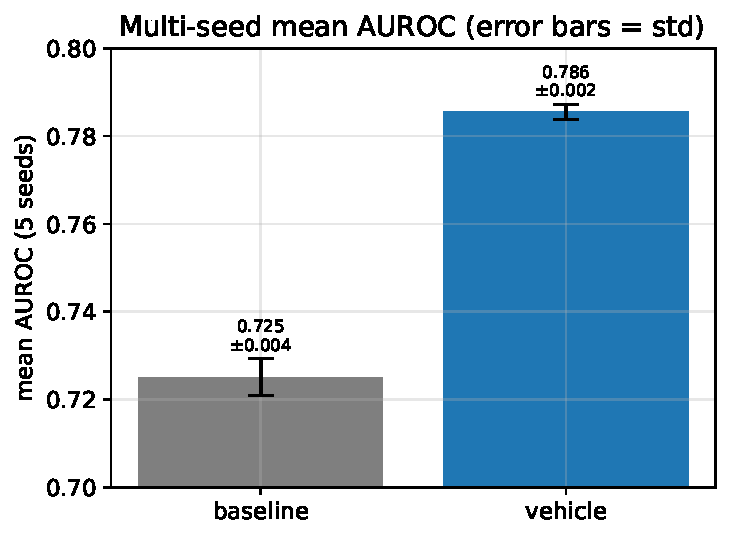
\includegraphics[width=0.40\textwidth]{res_multiseed.pdf}\hfill
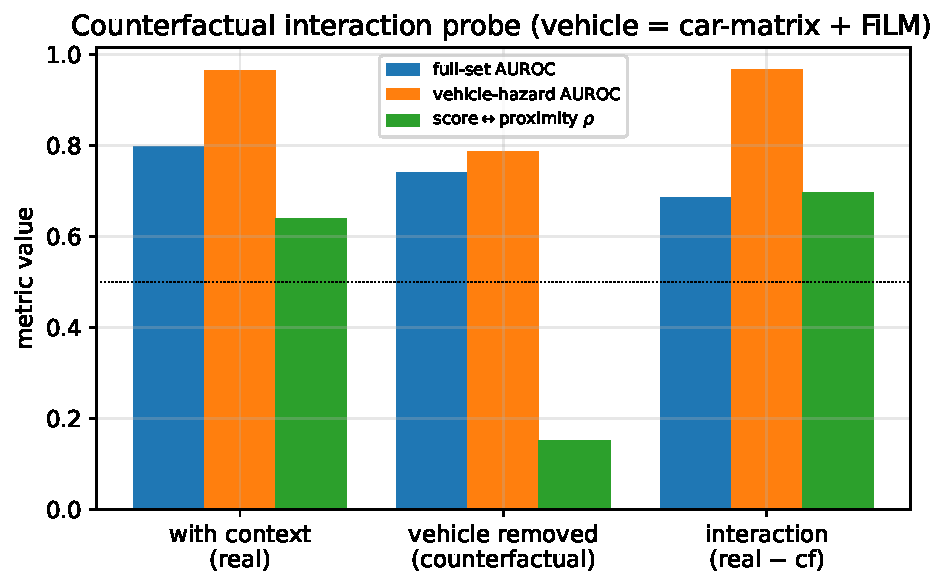
\includegraphics[width=0.58\textwidth]{res_counterfactual.pdf}
\caption{\textbf{Left:} multi-seed mean AUROC (error bars $=$ std over 5 seeds);
the baseline/car-matrix gap is large relative to the spread. \textbf{Right:}
counterfactual interaction probe. Removing the vehicle (zeroing the context)
collapses the model to near-baseline (full $0.74$, vehicle-hazard $0.79$,
$\rho{=}0.15$); the isolated interaction term (real$-$cf) is a near-perfect
\emph{vehicle-hazard} detector ($0.97$, $\rho{=}0.70$) yet a weak \emph{general}
detector ($0.69$) --- the signature of interaction, not constant presence.}
\label{fig:multiseed}
\end{figure}

\paragraph{Interaction vs.\ mere presence (primary result).} Overall AUROC
understates the contribution because it mixes anomaly types. We isolate the
interaction with a counterfactual: score each frame with the real context and
again with the context zeroed (vehicle ``removed''), then take the difference
(Figure~\ref{fig:multiseed}, right). Zeroing collapses the model to
near-baseline; the interaction term raises near-vehicle-hazard AUROC from $0.79$
to $\mathbf{0.97}$ and the score--proximity Spearman correlation from $0.16$ to
$\mathbf{0.70}$, while being only a weak general detector. A class-balanced
within-near-vehicle AUROC (bootstrap) of $\mathbf{0.62\,[0.59,0.66]}$ confirms
above-chance separation even after removing the $\sim$91\% label imbalance
(Table~\ref{tab:hazard}). Together these say the model fires on the
\emph{configuration}, not simply on the presence of a car.

\begin{table}[t]
\centering
\caption{Hazard-focused metrics (car-matrix\,+\,FiLM, $\sigma{=}0$). The
``interaction'' row is the counterfactual difference (real $-$ vehicle-removed).}
\label{tab:hazard}
\begin{tabular}{lccc}
\toprule
Variant & full-set AUROC & vehicle-hazard AUROC & score--proximity $\rho$ \\
\midrule
SeeKer baseline & 0.735 & 0.79 & 0.16 \\
with context (real) & 0.797 & 0.966 & 0.640 \\
vehicle removed (counterfactual) & 0.741 & 0.788 & 0.151 \\
\textbf{interaction (real $-$ cf)} & 0.687 & \textbf{0.967} & \textbf{0.698} \\
\midrule
\multicolumn{4}{l}{balanced near-vehicle AUROC (bootstrap): $0.62\,[0.59,0.66]$}\\
\bottomrule
\end{tabular}
\end{table}

\paragraph{Qualitative demo: predictions in action.}
Figure~\ref{fig:demo} traces both models' per-frame score on a single test clip in
which a cyclist (a hazard class) rides through a pedestrian entrance. Outside the
ground-truth anomaly window both models sit near zero (frames 48, 233). As the
hazard begins the car-matrix score jumps to its maximum and \emph{stays} elevated
through the vehicle-present interval (green ticks), whereas the baseline rises at
the onset but decays mid-event; at the vehicle-present peak (frame 180) the
oriented bicycle keypoints sit beside the pedestrians and our model scores $0.87$
versus the baseline's $0.49$. This is the intended behaviour --- the score
responds to the pedestrian--vehicle \emph{configuration}, not to motion alone. An
animated version is provided with the code (\texttt{demo\_detection.gif}).

\begin{figure}[t]
\centering
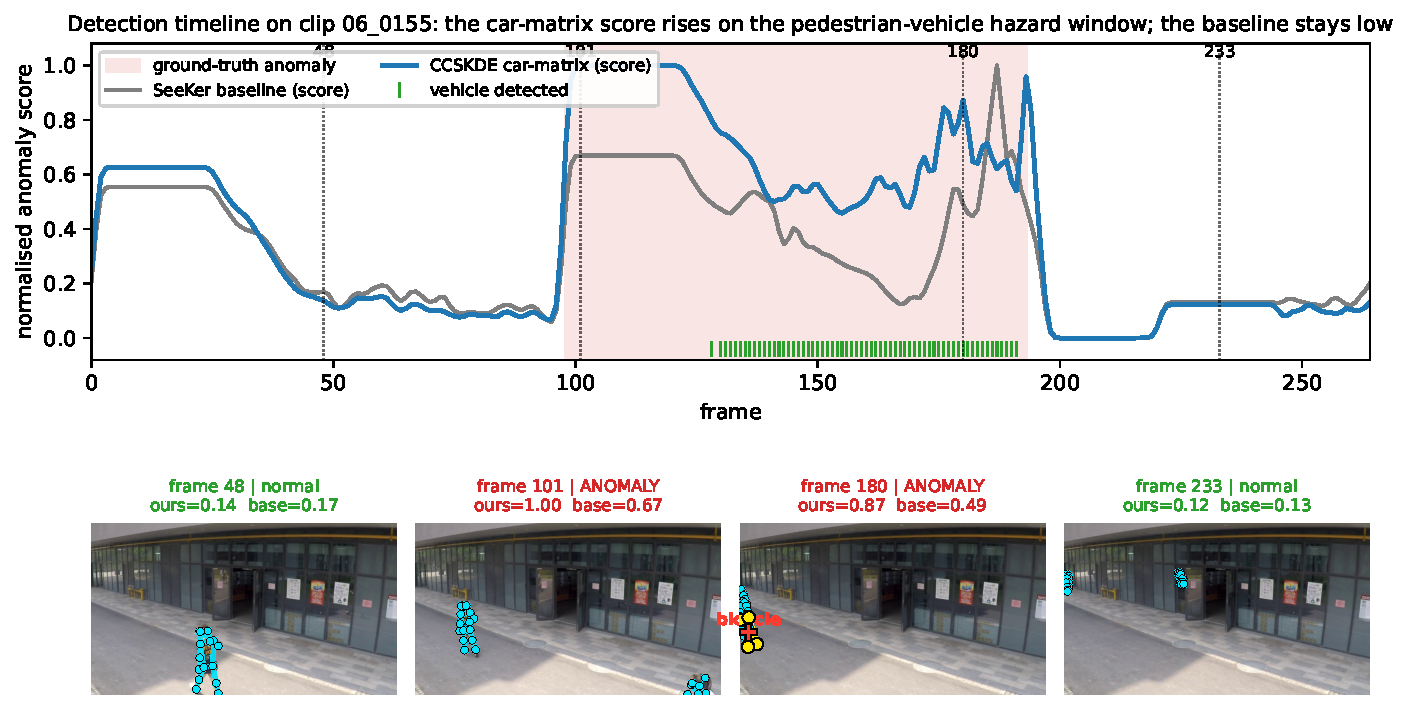
\includegraphics[width=0.99\textwidth]{demo_detection.pdf}
\caption{\textbf{Detection demo on clip 06\_0155.} \emph{Top:} normalised
per-frame anomaly score for the SeeKer baseline (grey) and our CCSKDE car-matrix
model (blue); the ground-truth anomaly window is shaded, green ticks mark frames
with a detected hazard vehicle. \emph{Bottom:} keyframes with the pedestrian
skeleton (cyan) and oriented vehicle keypoints (yellow/red), annotated with each
model's score. Our model stays high across the hazard; the baseline lags and
decays.}
\label{fig:demo}
\end{figure}

\paragraph{Operating-point sensitivity (an honest caveat).}
ShanghaiTech AUROC is sensitive to temporal smoothing $\sigma$
(Figure~\ref{fig:sigma}). Smoothing lifts the baseline ($0.781\!\rightarrow\!0.797$
at $\sigma{=}20$) but \emph{lowers} the car-matrix model
($0.802\!\rightarrow\!0.765$), because the interaction signal is temporally
punctate. At the baseline's best operating point the \emph{overall}-AUROC gap
narrows to $\sim$1 pp. We report this rather than tuning $\sigma$ in our favour:
the defensible claim is \emph{comparable overall AUROC plus a distinct interaction
signal}, not a global AUROC win.

\begin{figure}[t]
\centering
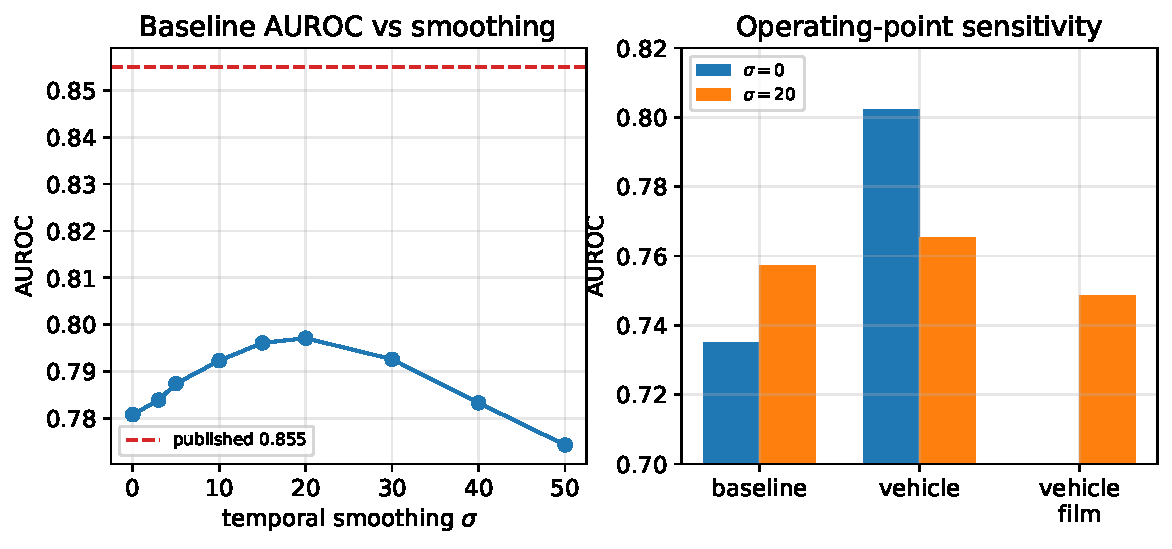
\includegraphics[width=0.92\textwidth]{res_sigma.pdf}
\caption{\textbf{Reproduction gap and operating-point sensitivity.} \emph{Left:}
baseline AUROC vs smoothing $\sigma$; smoothing accounts for $\sim$1.6 pp, leaving
a residual gap to the published $0.855$ (see text). \emph{Right:} at $\sigma{=}20$
the overall-AUROC advantage of the context model nearly vanishes.}
\label{fig:sigma}
\end{figure}

\paragraph{Reproduction gap.} Our baseline (mean $0.725$, best $0.797$ with
smoothing) sits below SeeKer's published $0.855$. We attribute the residual to
(i) the public code path used here scores only the last frame of each window via
\texttt{validate}; the full-window test-time scorer (\texttt{joint\_lnp\_full\_window})
that \texttt{test} calls is \emph{undefined} in the released snapshot, and (ii)
unspecified training/scoring details common to skeleton-VAD reproductions. All
our comparisons use one reproduced baseline and pipeline, so relative claims are
unaffected.

\paragraph{Efficiency.} The density models are lightweight: $2.24$/$2.97$/$6.22$\,M
parameters (baseline/car-matrix+FiLM/scene), $0.30$/$0.41$/$0.72$\,ms per batch
($>\!3\times10^{7}$ frame-scores/s on one RTX~5080). YOLO/AlphaPose are one-time
offline costs.

% =============================================================================
\section{Ablation Studies}
\label{sec:ablation}
Beyond the variant comparison of Tables~\ref{tab:single}--\ref{tab:suite}, we run
two controlled sweeps that isolate specific design choices (Table~\ref{tab:abl},
$\sigma{=}0$, single seed): the number of vehicles $M$ kept per frame, and the
agent ordering in the unified model.

\begin{table}[t]
\centering
\caption{Controlled ablations ($\sigma{=}0$, single seed). \emph{Top:} number of
vehicles $M$ in the car-matrix context. \emph{Bottom:} agent ordering in the
unified Scene-SKDE (vehicles-first = pedestrian conditioned on vehicles;
pedestrian-first removes that conditioning at identical capacity).}
\label{tab:abl}
\begin{tabular}{lccccc}
\toprule
Ablation & AUROC & AUPRC & EER$\downarrow$ & per-scene macro & veh-haz \\
\midrule
\multicolumn{6}{l}{\emph{Number of vehicles $M$ (car-matrix context)}}\\
\;\;$M{=}1$ & 0.799 & 0.720 & 0.283 & 0.757 & 0.958 \\
\;\;$M{=}2$ (default) & \textbf{0.802} & 0.720 & \textbf{0.270} & \textbf{0.770} & 0.950 \\
\;\;$M{=}3$ & 0.788 & 0.711 & 0.298 & 0.747 & 0.957 \\
\midrule
\multicolumn{6}{l}{\emph{Agent ordering (unified Scene-SKDE, joint read-out)}}\\
\;\;vehicles-first (default) & 0.782 & 0.690 & 0.301 & 0.729 & 0.952 \\
\;\;pedestrian-first & 0.779 & 0.684 & 0.300 & 0.726 & 0.949 \\
\bottomrule
\end{tabular}
\end{table}

\textbf{(i) Context value:} adding any context lifts mean AUROC by $+6$--$7$ pp and
improves all four frame-level metrics (Table~\ref{tab:suite}). \textbf{(ii) Number
of vehicles:} $M{=}2$ is the sweet spot; $M{=}1$ is close and $M{=}3$ is slightly
\emph{worse} on overall AUROC, AUPRC and per-scene macro --- on a pedestrian
campus a third nearby vehicle is rare, so the extra slot mostly contributes
zero-fill noise. \textbf{(iii) Agent ordering:} placing vehicles before vs.\ after
the pedestrian changes \emph{every} metric by $\le 0.3$ pp --- a near-wash. The
honest reading is that for the unified model it is the \emph{joint inclusion} of
vehicles in the density, more than the specific autoregressive order, that carries
the effect; the conditioning direction is a second-order factor once the
aggregate scene likelihood already sees the vehicle keypoints. \textbf{(iv)
Spatial alignment (shuffled control):} permuting the context across segments ---
identical parameter count, geometry misaligned --- drops the car-matrix best from
$0.802$ to $0.789$ and weakens every hazard metric (Table~\ref{tab:suite}); the
gap is the portion attributable to genuine spatial alignment, the remainder to the
regularising effect of a richer input. \textbf{(v) FiLM covariance:} the FiLM gate
yields the best AUPRC, the strongest vehicle-hazard AUROC and the strongest
score--proximity coupling (Table~\ref{tab:suite}). \textbf{(vi) Representation:}
the oriented car-matrix and the simple proximity vector are comparable on overall
AUROC, but the oriented geometry gives a clearly better per-scene macro
($0.770$ vs $0.751$), i.e.\ geometry aids cross-scene generalisation.
\textbf{(vii) Temporal smoothing} (Figure~\ref{fig:sigma}) remains the most
influential test-time hyper-parameter.

% =============================================================================
\section{Limitations}
\label{sec:limitations}
\textbf{(1) Single dataset.} We evaluate only on ShanghaiTech; SeeKer also uses
UBnormal and MSAD-HR. \textbf{(2) Presence vs.\ interaction not fully
disentangled.} On ShanghaiTech a near-vehicle frame is $\sim$91\% anomalous
(Fig.~\ref{fig:eda2}); the counterfactual is strong evidence of
configuration-dependence, but a definitive separation needs a benchmark where
vehicles are sometimes normal (e.g.\ MSAD-HR). \textbf{(3) Overall-AUROC gain is
operating-point-sensitive} (Fig.~\ref{fig:sigma}); we therefore foreground the
interaction metrics. \textbf{(4) Reproduction gap} to the published $0.855$.
\textbf{(5) Model capacity:} a first-order, diagonal-Gaussian, single-layer MADE
cannot represent higher-order multi-agent dynamics or multimodal normal motion.
\textbf{(6) Scene read-out:} the unified model is scored on pedestrian keypoints
for comparability, leaving vehicle-intrinsic hazards to a future joint read-out.

% =============================================================================
\section{Discussion}
\label{sec:discussion}
The clean finding is that an autoregressive keypoint density \emph{can} be
extended to multiple, heterogeneous agents without abandoning SeeKer's mechanism
or efficiency, and that doing so injects a measurable pedestrian--vehicle
interaction signal --- exactly the quantity a motion-only model is blind to. The
counterfactual analysis is, in our view, more convincing than a raw AUROC delta:
it shows the contribution is the \emph{vehicle's effect on the pedestrian
likelihood}, which behaves like interaction (configuration-dependent, strongly
proximity-coupled) rather than a presence prior. At the same time, the
operating-point study is a cautionary tale for skeleton-VAD comparisons: an
un-smoothed AUROC can flatter a model whose signal is temporally punctate. We
deliberately report the less favourable smoothed comparison.

% =============================================================================
\section{Future Directions}
\label{sec:future}
(1) \textbf{MSAD-HR / cross-dataset:} a setting with normal vehicles would
separate hazard from presence and test generalisation. (2) \textbf{Full
multi-seed} of every config with significance tests. (3) \textbf{Expressive
conditional:} replace the diagonal Gaussian with a normalizing-flow or diffusion
head (SeeKer's own ablation shows richer \emph{covariance} buys little, so
expressivity should come from the conditional). (4) \textbf{Universal keypoint
agents:} a promptable keypoint model (e.g.\ X-Pose) would let any human, animal,
or object become an agent in the same density --- a path to ``SKDE for anything
with keypoints'', including animal-behaviour and crowd anomalies. (5)
\textbf{Hazard anticipation:} roll out the density to score predicted
near-collisions (a learned TTC/PET surrogate).

% =============================================================================
\bibliographystyle{iclr2025_conference}
\begin{thebibliography}{99}

\bibitem[Deli{\'c} et~al.(2025)]{delic2025seeker}
Deli{\'c}, A., Gr{\v c}i{\'c}, M., \& {\v S}egvi{\'c}, S. (2025).
\newblock Sequential Keypoint Density Estimator: An Overlooked Baseline of
Skeleton-Based Video Anomaly Detection. In {\em ICCV} (Highlight).

\bibitem[Germain et~al.(2015)]{germain2015made}
Germain, M., Gregor, K., Murray, I., \& Larochelle, H. (2015).
\newblock MADE: Masked Autoencoder for Distribution Estimation. In {\em ICML}.

\bibitem[Hirschorn \& Avidan(2023)]{hirschorn2023normalizing}
Hirschorn, O., \& Avidan, S. (2023).
\newblock Normalizing Flows for Human Pose Anomaly Detection. In {\em ICCV}.

\bibitem[Morais et~al.(2019)]{morais2019messagepassing}
Morais, R., Le, V., Tran, T., Saha, B., Mansour, M., \& Venkatesh, S. (2019).
\newblock Learning Regularity in Skeleton Trajectories for Anomaly Detection in
Videos. In {\em CVPR}.

\bibitem[Markovitz et~al.(2020)]{markovitz2020graph}
Markovitz, A., Sharir, G., Friedman, I., Zelnik-Manor, L., \& Avidan, S. (2020).
\newblock Graph Embedded Pose Clustering for Anomaly Detection. In {\em CVPR}.

\bibitem[Ionescu et~al.(2019)]{ionescu2019object}
Ionescu, R.~T., Khan, F.~S., Georgescu, M.-I., \& Shao, L. (2019).
\newblock Object-Centric Auto-Encoders and Dummy Anomalies for Abnormal Event
Detection in Video. In {\em CVPR}.

\bibitem[Doshi \& Yilmaz(2025)]{complexvad2025}
Doshi, K., \& Yilmaz, Y. (2025).
\newblock ComplexVAD: Detecting Interaction Anomalies in Video. In {\em WACV}.

\bibitem[Wiederer et~al.(2022)]{wiederer2022anomaly}
Wiederer, J., Bouazizi, A., Troina, M., Kressel, U., \& Belagiannis, V. (2022).
\newblock Anomaly Detection in Multi-Agent Trajectories for Automated Driving.
In {\em CoRL}.

\bibitem[Perez et~al.(2018)]{perez2018film}
Perez, E., Strub, F., de~Vries, H., Dumoulin, V., \& Courville, A. (2018).
\newblock FiLM: Visual Reasoning with a General Conditioning Layer. In {\em AAAI}.

\bibitem[Dinh et~al.(2017)]{dinh2017realnvp}
Dinh, L., Sohl-Dickstein, J., \& Bengio, S. (2017).
\newblock Density Estimation Using Real NVP. In {\em ICLR}.

\bibitem[Kingma \& Dhariwal(2018)]{kingma2018glow}
Kingma, D.~P., \& Dhariwal, P. (2018).
\newblock Glow: Generative Flow with Invertible $1{\times}1$ Convolutions. In
{\em NeurIPS}.

\bibitem[Liu et~al.(2018)]{liu2018future}
Liu, W., Luo, W., Lian, D., \& Gao, S. (2018).
\newblock Future Frame Prediction for Anomaly Detection -- A New Baseline. In
{\em CVPR}.

\bibitem[Fang et~al.(2017)]{fang2017rmpe}
Fang, H.-S., Xie, S., Tai, Y.-W., \& Lu, C. (2017).
\newblock RMPE: Regional Multi-Person Pose Estimation. In {\em ICCV}.

\bibitem[Ultralytics(2024)]{ultralytics2024yolov11}
Ultralytics. (2024). YOLOv11. \url{https://github.com/ultralytics/ultralytics}.

\end{thebibliography}

\end{document}
